\section{处理辐射积分}\label{sec:处理辐射积分}

渲染中最频繁的任务之一就是求辐射度量数量的积分。
本节中,我们将介绍可以使该任务更简单的一些技巧。
为了说明这些技术的运用,我们将以计算在一点处的辐射照度为例。
在曲面法线为$\bm n$的点$\bm p$处的辐射照度取决于
方向集$\Omega$上的辐射亮度即
\begin{align}\label{eq:5.4}
    E({\bm p},{\bm n})=\int\limits_{\Omega}{L_{\mathrm{i}}({\bm p},{\bm\omega})|\cos\theta|\mathrm{d}\bm\omega}\, ,
\end{align}
其中$L_{\mathrm{i}}({\bm p},{\bm\omega})$是入射辐亮度函数(\reffig{5.12})
而该积分中项$\cos\theta$取决于辐射亮度定义中的项$\mathrm{d}A^{\perp}$。
$\theta$度量$\bm\omega$和曲面法线$\bm n$之间的夹角。
辐射照度通常在关于给定曲面法线$\bm n$的半球方向$H^2(\bm n)$上算出。
\begin{figure}[htbp]
    \centering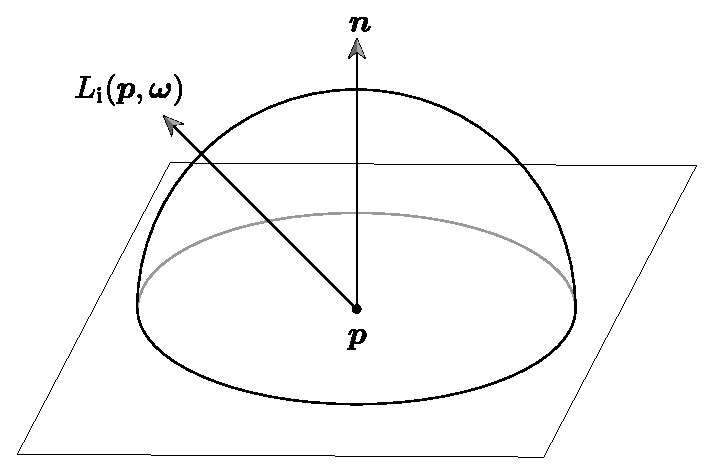
\includegraphics[width=0.5\linewidth]{chap05/Irradiancefromradiance.eps}
    \caption{点$\bm p$处的辐射照度由辐射亮度乘以在该点上整个上半球入射方向余弦的积分得到。}
    \label{fig:5.12}
\end{figure}

\subsection{投影立体角上的积分}\label{sub:投影立体角上的积分}
